\chapter{Casos de estudio}

Ya hemos presentado el verificador de modelos MC2 y el lenguaje de descripción asociado al mismo. Es hora de observar algunos ejemplos concretos de uso de esta herramienta, y ese es el propósito de este capítulo final. Veremos como modelar tres clásicos juegos solitarios de lógica y estrategia, y analizaremos hasta que punto es viable describir manualmente el modelo con esta versión básica de MC2.

\section{Cruce del rio}

Existen muchas versiones de este problema, nosotros modelaremos una de las versiones mas conocidas \cite{Hadley:12}. El problema es el siguiente, un granjero va a comprar un zorro, un ganso y una bolsa de frijoles. Mientras vuelve a su casa, se encuentra con que debe cruzar un rio, para lo cuál alquila un bote. El granjero solo puede llevar una de sus compras en el barco. Si se deja al zorro con el ganso, el zorro se lo va a comer, y si se deja al ganso con la bolsa de frijoles, este se va a comer los frijoles. El desafio del granjero es el de llevar todas sus compras intactas al otro lado del rio. El problema consiste entonces en elegir sabiamente que compras trasladar en cada viaje.

La descripción MC2 para el modelo de este problema esta en la figura \ref{fig:river}.Para modelarlo declaramos cuatro pares de proposiciones atómicas, uno para cada compra y otro para el barco/granjero, las proposiciones marcadas con $1$ hacen referencia a que estan del lado $origen$ del rio, y las marcadas con $2$ hacen referencia a que estan del lado $destino$ del rio. En cuanto a las reglas, hay dos grupos de reglas a tener en cuenta para describir el comportamiento del sistema, por un lado se describe lo que pasa cuando se dejan juntos objetos incompatibles (por ejemplo, zorro y ganso), por otro lado tenemos las reglas que definen la acción de viajar de un lado del rio al otro (se puede viajar solo o acompañado por un solo objeto). En este caso, en el estado inicial queremos que valga que tanto el granjero/bote como el zorro, el ganso y los frijoles estan del lado $origen$ del rio. Por último, la propiedad que queremos verificar es si existe alguna forma de que, siguiendo las reglas, puedan estar el zorro, el ganso y los frijoles en el lado $destino$ del rio. En la figura \ref{fig:riverobdd} está el OBDD que representa al modelo.

\begin{figure}[H]
  \centering
  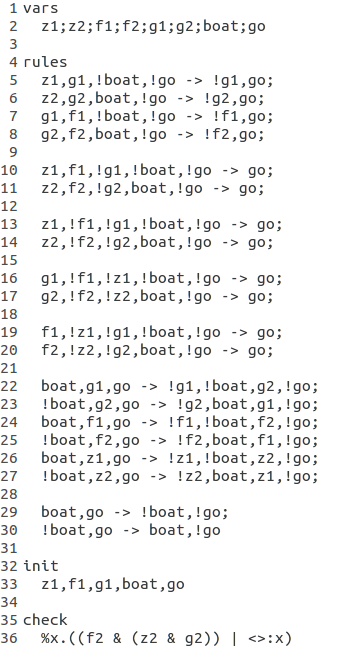
\includegraphics[width=0.6\textwidth]{Figures/rivercross.png}
  \caption{Descripción de modelo del problema del cruce del rio.}
  \label{fig:river}
\end{figure}

\begin{figure}[H]
  \centering
  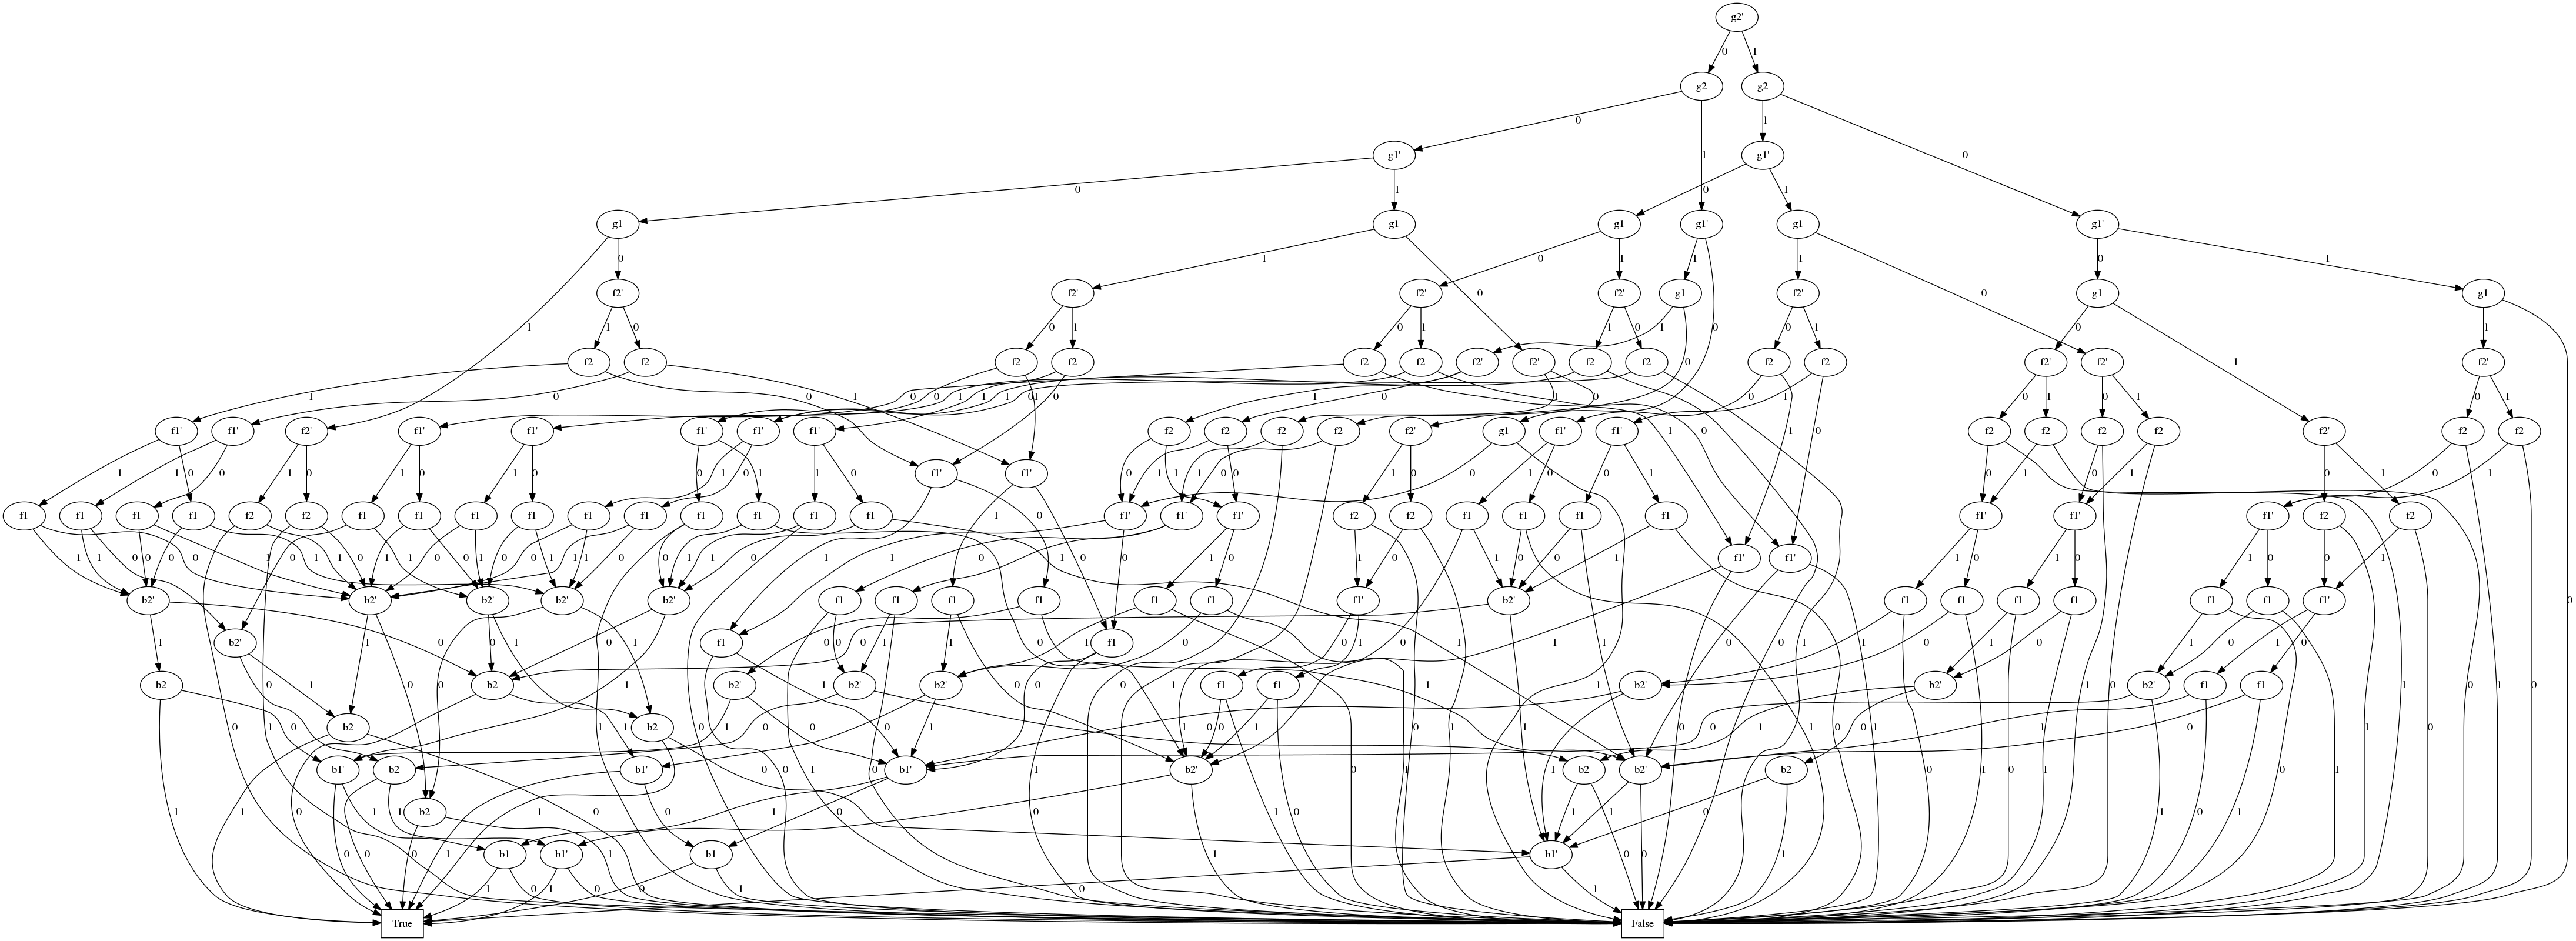
\includegraphics[width=0.9\textwidth]{Figures/riverobdd.png}
  \caption{OBDD para el modelo del cruce del rio.}
  \label{fig:riverobdd}
\end{figure}

\section{1,2,3, Coloca otra vez}

Se trata de un juego de tipo solitario.
Se parte de una estrella de 5 puntas.
Partiendo de uno de los huecos en los que no haya una ficha previamente colocada, contaremos tres posiciones consecutivas sobre una de las aristas que contienen la posición de partida. Tras ello, colocaremos una ficha en la tercera posición (la última del conteo).
El conteo puede pasar por una posición en la que haya ficha, pero no puede iniciarse en una posición con ficha.
El juego estará resuelto cuando se hayan colocado 9 fichas. \cite{Juegos:11} \ref{fig:pentagrama} \ref{fig:estrella}

\begin{figure}[H]
  \centering
  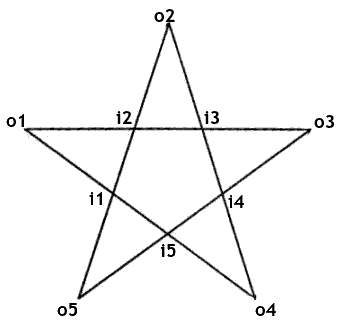
\includegraphics[width=0.5\textwidth]{Figures/pentagram.png}
  \caption{Pentagrama de 1,2,3 Coloca otra vez.}
  \label{fig:pentagrama}
\end{figure}

\begin{figure}[H]
  \centering
  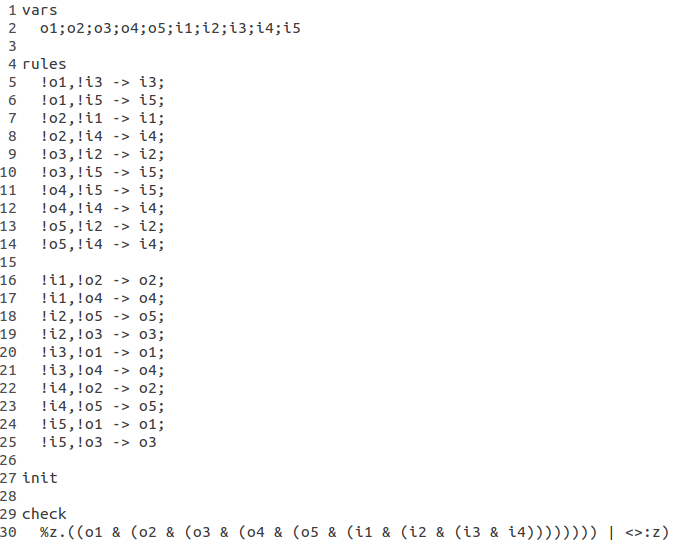
\includegraphics[width=1\textwidth]{Figures/estrella.png}
  \caption{Descripción de modelo del problema de 1,2,3 Coloca otra vez.}
  \label{fig:estrella}
\end{figure}

\section{Ranas saltarinas}

Se trata de un juego de tipo solitario. Para un sólo jugador.
Se parte de una tira de papel dividida en siete casillas.
La posición inicial es la indicada con tres fichas azules y tres rojas colocadas como en la figura de abajo.
El objetivo del juego consiste en permutar las posiciones de las fichas azules y rojas. Es decir, las azules han de pasar a ocupar las posiciones de las rojas y viceversa. Para ello son válidos los siguientes movimientos:
a) Una ficha puede moverse a un lugar contiguo, si éste está vacío.
b) Una ficha junto a otra de distinto color puede saltar por encima de ella si el salto (por encima de una sola ficha) le lleva a una casilla vacía.
c) Son válidos tanto los movimientos hacia atrás como hacia adelante.
¿Cuál es el mínimo número de movimientos necesarios para resolverlo?.
Si jugamos con n fichas de cada color, dejando una casilla vacía, ¿cuál será ahora ese número mínimo de movimientos?.
¿Y si jugamos con n fichas de cada color, pero dejando m casillas vacías en el centro?.
¿Puedes demostrar los resultados obtenidos? \cite{Juegos:11} \ref{fig:ranas}

\begin{figure}[H]
  \centering
  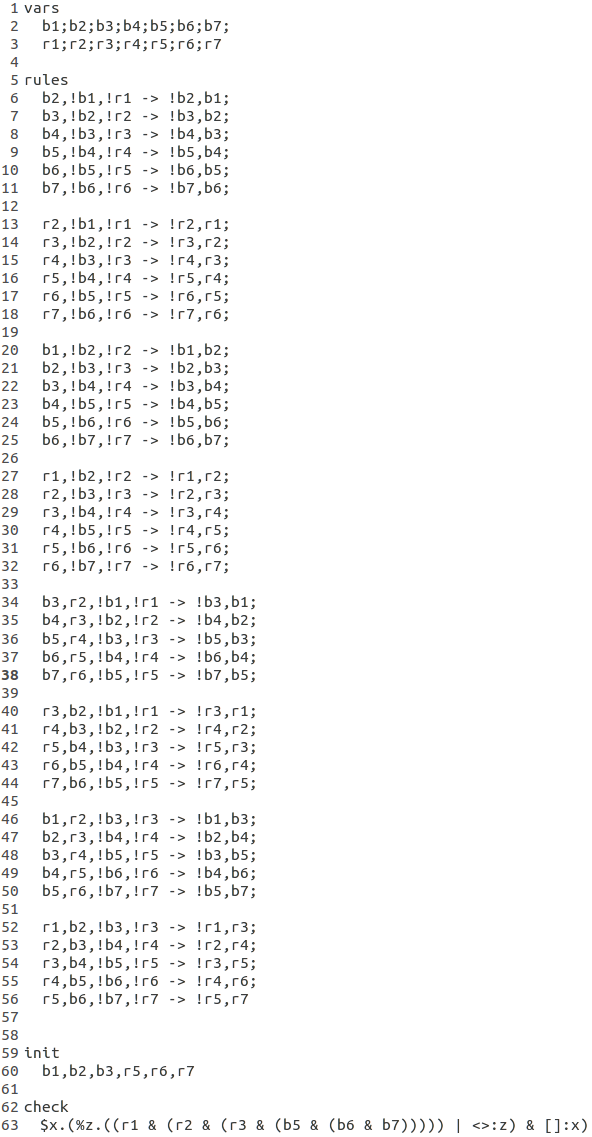
\includegraphics[width=0.5\textwidth]{Figures/ranas.png}
  \caption{Descripción de modelo del problema de las ranas saltarinas.}
  \label{fig:ranas}
\end{figure}

\chapter*{Conclusion}